\chapter{Software Installation and Setup} \labchap{software_guide}

The Thetis instrumentation board is an open source all-in-one inertial data logger for three dimensional bodies.
It was designed and developed for a Master's thesis in Ocean Engineering and the Florida Institute of Technology from 2020 to 2023.
This repository is the firmware used on that board to capture sensor measurements and compute body orientation and log all the appropriate data.

\section{Installing the Development Environment}
This firmware was developed in Microsoft Visual Studio Code using the PlatformIO extension on Windows 10 for compilation and uploading.
To automatically install and initialize the environment, download the initialization scripts\footnote{\url{https://github.com/Legohead259/Thetis-Firmware/tree/master/scripts}} and execute \lstinline[style=customInline]|1-dev_environment_setup.bat| as an administrator, following the on-screen prompts.
It will go through the steps discussed in the following sections.

\subsection{Step 1: Install VS Code and git VCS}
Download VisualStudio Code\footnote{\url{https://code.visualstudio.com/download}} from Microsoft and install it following the on-screen prompts.
Alternatively, it can be installed from the command prompt as an administrative user via:

\begin{bash}
    winget install -e -id Microsoft.VisualStudioCode
\end{bash}

Then, download git\footnote{\url{https://git-scm.com/downloads}} and install it using the on-screen prompts.
You should keep everything to the default value except for the text editor.
I would recommend Nano over Vim (unless you know how to exit Vim).
This can also be installed from the command prompt via:

\begin{bash}
    winget install -id Git.Git -e --source winget
\end{bash}

Finally, \textbf{for developers only} download the GitHub CLI client\footnote{\url{https://cli.github.com/}} and install it.
This can be done from the command prompt via:

\begin{bash}
    winget install --id=GitHub.cli -e
\end{bash}

Close and reopen any command prompt windows and test your installations with the following command:

\begin{bash}
    code --version && git  --version && gh --version
\end{bash}

If all the software has been installed correctly, you should see a short output similar to this:

\begin{bash}
    1.83.1
    f1b07bd25dfad64b0167beb15359ae573aecd2cc
    x64
    git version 2.42.0.windows.2
    gh version 2.36.0 (2023-10-03)
    https://github.com/cli/cli/releases/tag/v2.36.0
\end{bash}

\subsection{Step Two: Install Extensions for VSCode}
If all the software has been installed correctly, we can now install the required extensions. 
PlatformIO \footnote{\url{https://platformio.org/}} is an advanced development environment for embedded systems.
It has excellent integration with VSCode that allows for large projects to be more easily managed and programmed.
To install PlatformIO through the VSCode GUI, open the application and look for the ``Extensions'' tab on the left-hand side (in red).
Select it, then search for PlatformIO in the marketplace (green).
Do the same for CPP Tools (blue) if not already installed.

\begin{figure}[h!]
    \centering
    \subfloat[PlatformIO extension in VSCode]{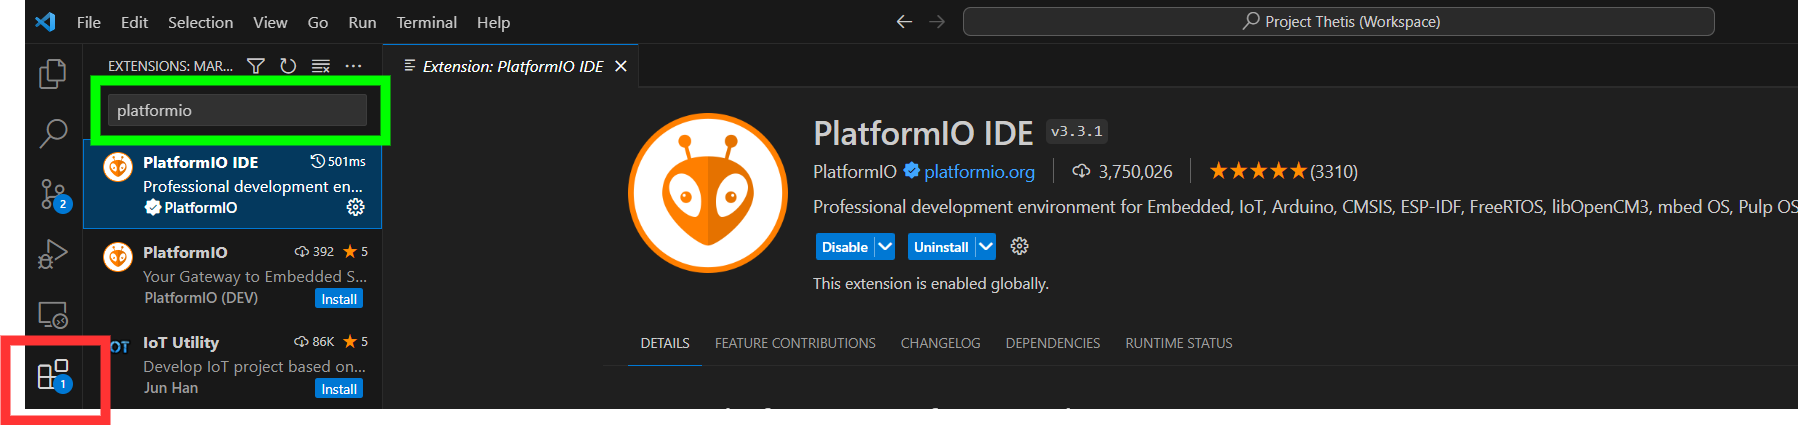
\includegraphics[width=\textwidth]{appendices/software_guide/vscode_extension_platformio.png}} \hskip3ex
    \subfloat[C++ tools extension in VSCode]{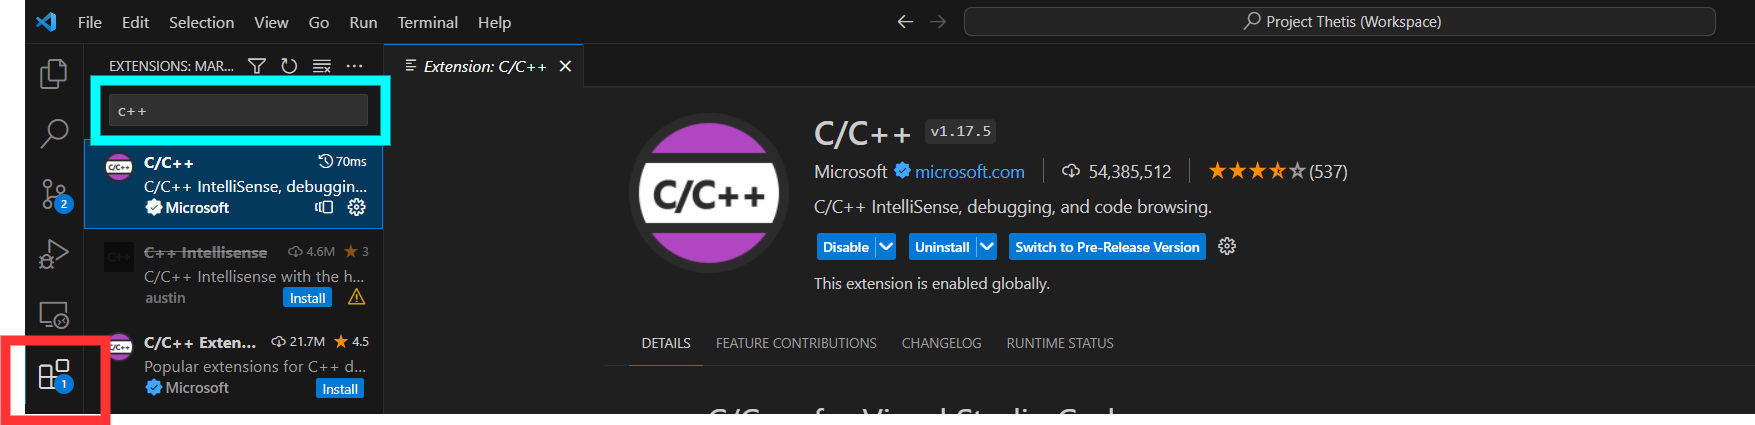
\includegraphics[width=\textwidth]{appendices/software_guide/vscode_extension_cpptools.png}}
    \caption{Installation of extensions in VSCode}
    \labfig{vscode_extensions}
\end{figure}

Alternatively, these can be installed in the command prompt with:

\begin{bash}
    code --install-extension platformio.platformio-ide
    code --install-extension ms-vscode.cpptools
\end{bash}

\subsection{Step Three: Clone the Thetis-Firmware Repository to a Directory}
Once the applications have been installed, you can clone the Thetis-Firmware repository \cite{Thetis-Firmware} to your local machine.
Navigate to a directory you want to install the firmware onto (e.g. ``C:\textbackslash USER\textbackslash Desktop\textbackslash Thetis\textbackslash'') and open that location in a command prompt.
(\textit{Hint}: You can right-click within the folder and select ``Open Git Bash Here'' option.)
Then, execute the command:

\begin{bash}
    git clone https://github.com/Legohead259/Thetis-Firmware.git
\end{bash}

\begin{figure}[h!]
    \centering
    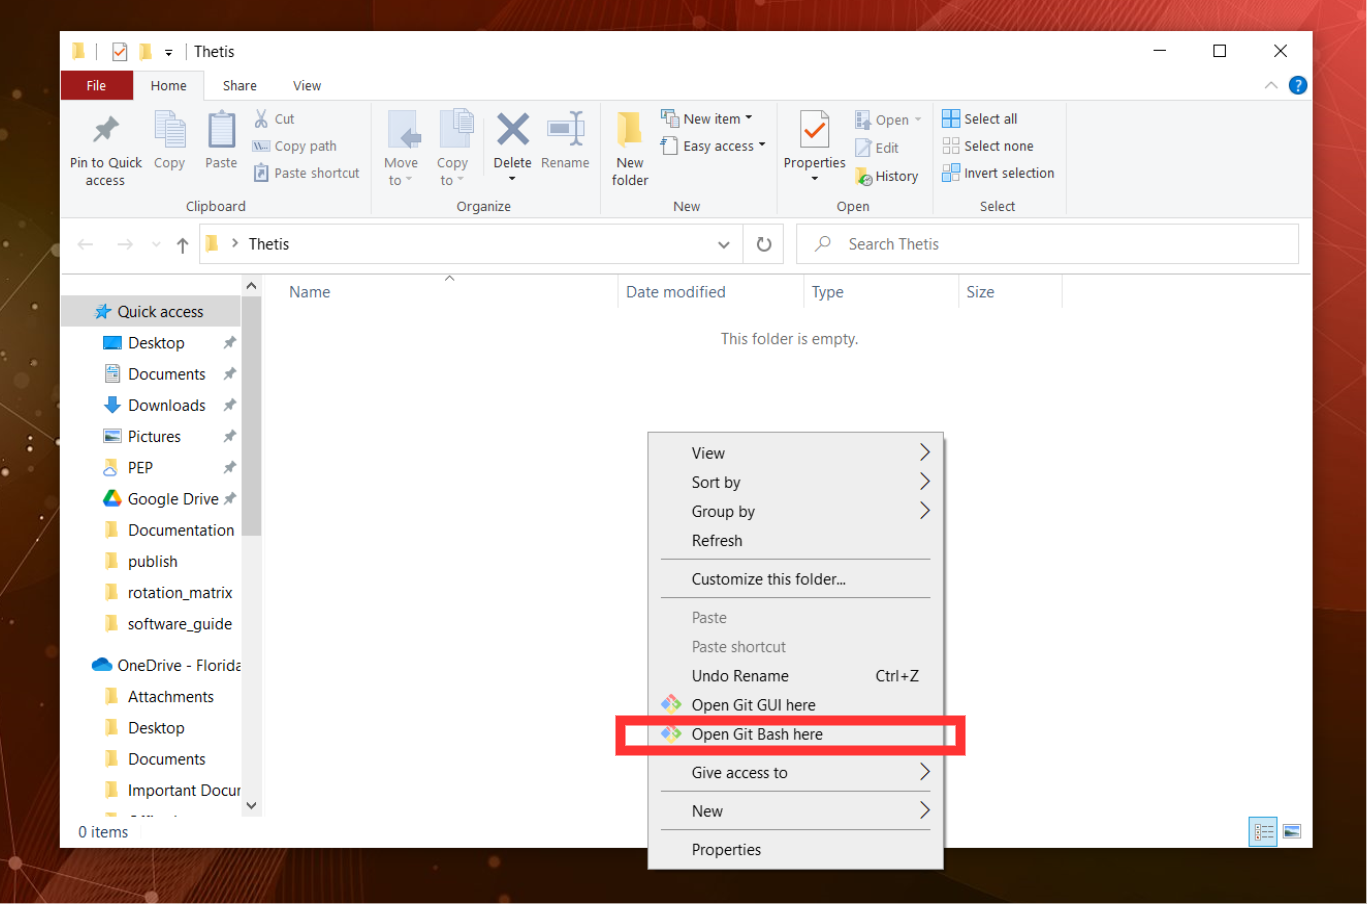
\includegraphics[height=3.5in]{appendices/software_guide/file_explorer_git_bash.png}
    \caption{Opening git bash in Windows File Explorer}
    \labfig{file_explorer_git}
\end{figure}

Once the folder is cloned, open it in the command prompt and initialize the submodule repositories with the command:

\begin{bash}
    chdir Thetis-Firmware && git submodule update --init --recursive
\end{bash}

\subsection{Step Four: Check Proper PIO and Firmware Installation}
Once the previous command finishes, execute the following command to compile the firmware and ensure everything is installed properly:

\begin{bash}
    %USERPROFILE%\.platformio\penv\Scripts\platformio.exe run -e thetis_revf5
\end{bash}

If the code successfully compiles, you should see an output like this:

\begin{figure}[h!]
    \centering
    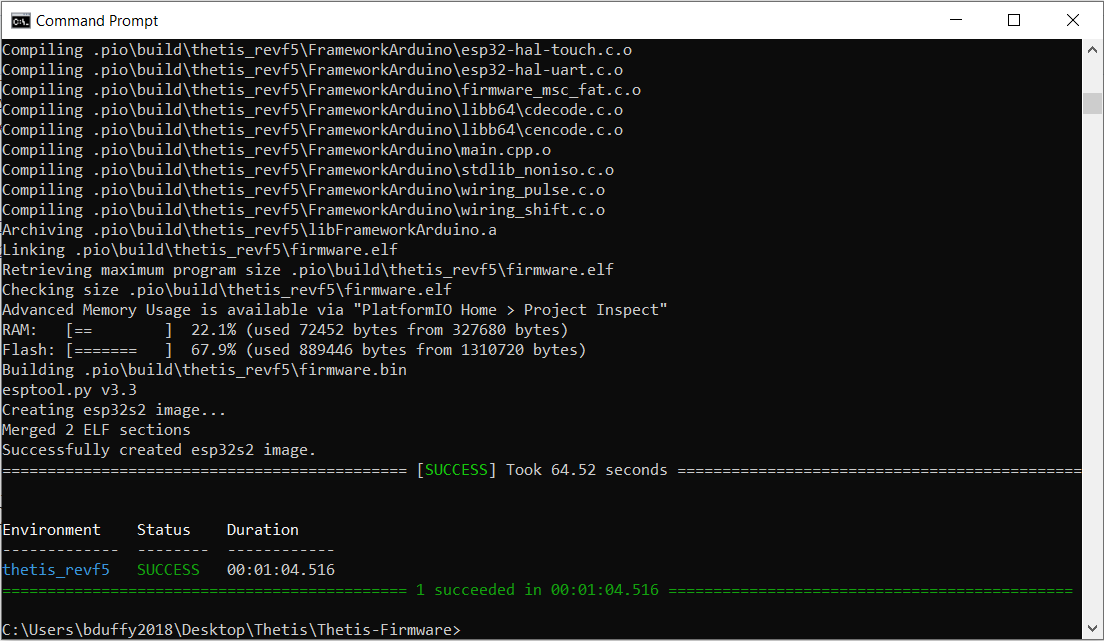
\includegraphics[height=3in]{appendices/software_guide/platformio_compile_test.png}
    \caption{Output from a successful PlatformIO compile}
    \labfig{platformio_compile_test}
\end{figure}

If the command prompt shows that output, congratulations!
You have successfully installed the basic development environment to upload new code to Thetis.

\section{Advanced Development Environment Setup}
\textbf{FOR DEVELOPERS ONLY}
Now that the development environment is set up, you must fork the firmware repositories to your own GitHub account.
This will preserve the original source code and allow you to use GitHub to track any changes you make.
Substantial changes can be made to the source repository through an appropriate pull request\footnote{\url{https://docs.github.com/en/pull-requests/collaborating-with-pull-requests/proposing-changes-to-your-work-with-pull-requests/creating-a-pull-request-from-a-fork}}.

To automatically configure the git environment, you can download and execute the \lstinline[style=customInline]|git_setup.bat| script.
Or, you can follow along with the upcoming sections.

\subsection{Configure Git Parameters}
Open a new command prompt in the cloned \lstinline[style=customInline]|Thetis-Firmware/| folder.
Before starting anything, we need to tell git CLI who you are.
First, we call the following commands, replacing the \lstinline[style=customInline]|GITHUB_USER| and \lstinline[style=customInline]|GITHUB_EMAIL| with those for your GitHub account:

\begin{bash}
    git config --global user.name GITHUB_USER
    git config --global user.email GITHUB_EMAIL
\end{bash}

Then, we will authorize the GitHub CLI client to make requests to the GitHub servers on your behalf:

\begin{bash}
    gh auth login -p "https" -w
\end{bash}

This will give you a one-time passcode and ask to open a web browser to log into GitHub.

\subsection{Fork Repositories and Reconfigure Submodules}
Once you authorize GitHub CLI to use your account, we can begin forking the firmware repositories.
First, execute the commands:

\begin{bash}
    gh repo fork https://github.com/Legohead259/Thetis-Firmware.git --remote=true
    gh repo fork https://github.com/Legohead259/ThetisLib.git --remote=true
    gh repo fork https://github.com/Legohead259/Fusion-Arduino.git --remote=true
    gh repo fork https://github.com/Legohead259/Timer-Events-Arduino.git --remote=true
    gh repo fork https://github.com/Legohead259/xioAPI-Arduino.git --remote=true
\end{bash}

Then, we must redirect the submodule URLs to the new repositories.
Navigate to the \lstinline[style=customInline]|Thetis-Firmware/| root directory and call:

\begin{bash}
    git submodule set-url lib/ThetisLib https://github.com/GITHUB_USER/ThetisLib.git
\end{bash}

Again, replacing \lstinline[style=customInline]|GITHUB_USER| with your GitHub username.
Then, navigate to the \lstinline[style=customInline]|Thetis-Firmware/lib/ThetisLib/| folder and execute the following:

\begin{bash}
    git submodule set-url src/fusion https://github.com/GITHUB_USER/Fusion-Arduino.git
    git submodule set-url timing https://github.com/GITHUB_USER/Timer-Events-Arduino.git
    git submodule set-url src/xioAPI https://github.com/GITHUB_USER/xioAPI-Arduino.git
    git submodule sync
\end{bash}

Return to the \lstinline[style=customInline]|Thetis-Firmware/| root directory and execute the submodule sync command again:

\begin{bash}
    git submodule sync
\end{bash}

This will redirect all submodule commands to your newly forked repositories and will allow you to make changes to any part of the firmware.
You should now have your own dedicated git environment to modify Thetis and save those changes.
